\documentclass[upright, contnum]{umemoria}
\depto{DEPARTAMENTO DE INGENIERÍA ELÉCTRICA}
\author{ALEXIS DANILO YÁÑEZ INOSTROZA}
\title{SISTEMA CONTEXT AWARE PARA LA DESCICIÓN DE MECANISMO DE DISEMINACIÓN EN REDES VEHICULARES AD-HOC}
\auspicio{}
\date{MAYO 2017}
\guia{SANDRA CÉSPEDES UMAÑA}
\carrera{MAGÍSTER EN CIENCIAS DE LA INGENIERÍA MENCIÓN ELÉCTRICA}
\memoria{TESIS PARA OPTAR AL GRADO DE}
\comision{NOMBRE1 APELLIDO1}{NOMBRE2 APELLIDO2}{\ }

\usepackage{lipsum}

\usepackage[utf8]{inputenc}
%\usepackage[T1]{fontenc}

\begin{document}

\frontmatter
\maketitle

\begin{abstract}
{\lipsum[1-4]}
\end{abstract}

\begin{dedicatoria} % opcional
Una dedicatoria corta. Por ejemplo, \emph{A los creadores de U-Campus}
\end{dedicatoria}

\begin{thanks} % opcional
\lipsum[1-2]
\end{thanks}
\cleardoublepage

\tableofcontents
\listoftables % opcional
\listoffigures % opcional

\mainmatter
1 Introduction 1
1.1 General background . . . . . . . . . . . . . . . . . . . . . . . . . . . . . . . . 1
1.2 Specific background . . . . . . . . . . . . . . . . . . . . . . . . . . . . . . . . 2
1.3 Hypotheses . . . . . . . . . . . . . . . . . . . . . . . . . . . . . . . . . . . . 2
1.4 Main objective . . . . . . . . . . . . . . . . . . . . . . . . . . . . . . . . . . 3
1.5 Specific objectives . . . . . . . . . . . . . . . . . . . . . . . . . . . . . . . . . 3
1.6 Structure of the thesis . . . . . . . . . . . . . . . . . . . . . . . . . . . . . . 4
2 State of the art 5
2.1 Spatial estimation: Kriging interpolator . . . . . . . . . . . . . . . . . . . . . 5
2.2 Multiple-point Simulation . . . . . . . . . . . . . . . . . . . . . . . . . . . . 7
2.2.1 SNESIM algorithm . . . . . . . . . . . . . . . . . . . . . . . . . . . . 9
2.3 Sparse Regularization . . . . . . . . . . . . . . . . . . . . . . . . . . . . . . . 10
2.3.1 Sparse and compressible representation . . . . . . . . . . . . . . . . . 10
2.3.2 Basics of RIPless Compressed Sensing theory . . . . . . . . . . . . . . 12
2.3.3 Sparse regularization with support prior knowledge . . . . . . . . . . 14
2.3.4 Compressed sensing in geoscience . . . . . . . . . . . . . . . . . . . . 16
3 Methodology 18
3.1 Problem Statement . . . . . . . . . . . . . . . . . . . . . . . . . . . . . . . . 18
3.2 Statistical support and weighting set definition . . . . . . . . . . . . . . . . . 19
3.3 Experimental setting . . . . . . . . . . . . . . . . . . . . . . . . . . . . . . . 22
4 Experimental results 24
4.1 Weighting matrix variability . . . . . . . . . . . . . . . . . . . . . . . . . . . 24
4.2 Analysis of model complexity . . . . . . . . . . . . . . . . . . . . . . . . . . 26
4.3 Scale variability and thresholding stage . . . . . . . . . . . . . . . . . . . . . 27
4.4 Multiscale averaging reconstruction and comparison with other methods . . . 31
5 Conclusion 38
5.1 Future Work . . . . . . . . . . . . . . . . . . . . . . . . . . . . . . . . . . . . 39
References 4
\chapter{Introducción}
    En este capitulo se presenta a modo de introducción al trabajo realizado, la motivación, antecedentes, descripción del problema, objetivos, metodología y las herramientas que se utilizan para dar forma al trabajo. Estas secciones pretenden bosquejar un marco donde se concibe y desarrolla el problema principal, con el objetivo de facilitar la comprensión del trabajo expuesto posteriormente.
    
\section{Motivación Y Antecedentes}

Los nuevos avances en tecnologías de información y comunicaciones se han expandido a diversas áreas, gracias a un crecimiento explosivo de dispositivos que pueden ser introducidos en diversos rubros de la producción y actividad humana.  Sin duda alguna que estos avances han presentado grandes ventajas que antes eran impensadas, siendo las redes inalámbricas uno de los descubrimientos más importantes que aportan un sinfín de beneficios, gracias a que prescinden de cableado y permiten movilidad de los terminales o nodos, reduciendo los costos de producción y permitiendo una comunicación versátil. 

Según datos de la Organización Mundial de la Salud (OMS) los accidentes de tránsito son la causa principal de muerte en el grupo de 15 a 29 años de edad. Más del $90\%$ de las muertes relacionadas con accidentes de tránsito se producen en países de ingresos medios o bajos, a pesar de que estos cuentan aproximadamente con el $50\%$ del parque automotriz mundial. La mitad de las personas que mueren por esta causa en todo el mundo son ``usuarios vulnerables de la vía pública", es decir: peatones, ciclistas y motociclistas \cite{GSRRS}.

Las redes vehiculares VANETs (\textit{Vehicular Ad-Hoc Networks}) han surgido como una de las soluciones más prometedoras para reducir los accidentes de transito y mejorar la eficiencia en sistemas de transporte inteligentes (\textit{Inteligent Transportation Systems (ITS)}). Éstos sistemas pueden soportar una gran variedad de aplicaciones, que buscan dar solución a problemas que surgen en el contexto del transporte vehicular \cite{Bi2017}, que además, son producto de las sociedades modernas. En resumen los grandes problemas asociados al transporte son: 

\begin{itemize}
\item Alta tasa de mortandad a causa de accidentes vehiculares \cite{GSRRS}.
\item Congestión de tráfico en ciudades altamente pobladas.
\item Altas emisiones de $CO_2$.   
\item Peligro frente a condiciones climáticas adversas.
\end{itemize} 

Estos problemas pueden ser abordados desde muchos enfoques. Las redes vehiculares pueden ayudar a sopesar estos problemas, sin embargo, su implementación posee aún grandes desafíos. Por lo cual, para que este tipo de tecnologías sea verdaderamente un aporte para solucionar problemáticas transversales, se necesita que su desempeño sea robusto y eficiente, en concordancia a los requerimientos de cada aplicación. 

Unas de las aplicaciones mas prometedoras tiene relación al envío de mensajes de alerta, para poder notificar de manera rápida y eficiente, eventos de importancia sobre el contexto vehicular (por ejemplo: colisiones, condiciones climáticas adversas, mal comportamiento de conductores, etc.) para de esta manera, los conductores puedan tomar una decisión para evitar posibles accidentes. Sin embargo estas aplicaciones tienen un mal comportamiento en escenarios en donde existen muchos vehículos o nodos, debido a la saturación del canal de comunicación.

Frente a lo expuesto, se hace imperante dar solución a las falencias que puedan tener las aplicaciones basadas en redes vehiculares, para que sean capaces de dar una respuesta contundente y robusta frente a los problemas ya mencionados.

%que  abordan los problemas de accidentes en las rutas, como también esquemas de pelotón basados en \textit{``Cooperative Adaptive Cruise Control"} (CACC) que contribuyen al uso eficiente de combustibles y a reducir los tiempos de viaje [3][4].
%
%
%Uno de los campos más promisorios corresponde al transporte, que a través de las VANETs (Vehicular Ad-hoc Networks) o Redes Vehicualers Ad-hoc en español. hace posible la confección de aplicaciones en aspectos como la seguridad, confort, congestión de transito, semáforos inteligentes entre otras. Este tipo de aplicaciones se enmarcan en lo que se conoce como SmartCities que reúne este tipo de aplicaciones, que se orientan en dar solución a problemáticas relacionadas con el transito y el desplazamiento inteligente de móviles dentro de la ciudad. De esta forma se puede reducir el consumo de combustible, tiempos de viajes, ofrecer mayor seguridad, disminuir la emisión de combustibles fósiles etc. Problemas que son producto de las actividades de la sociedad del siglo XXI, que día a día exige mayor eficiencia y rapidez pero de manera sustentable, en concordancia de la toma de conciencia y de los efectos colaterales que pueden producir ciertas actividades.
%Las aplicaciones en tiempo real presentan altos desafíos en las VANETs, dado que cada procedimiento debe ser muy preciso, y tiene que ser ejecutado en el menor tiempo posible, para de esta forma obtener una respuesta adecuada para que pueda transmitir seguridad y confianza al usuario. Además, estas redes suelen tener una arquitectura P2P lo cual dificulta procesos de enrutamiento, identificación, entre otras.
%Una de las formas en que se aborda este problema es a través de esquemas cooperativos donde los vehículos comparten la información que generan. De esta forma se pueden reducir errores en la adquisición de datos de cada nodo en particular. Sin embargo esto conlleva un uso del canal de comunicación, no tan solo de la información de interés, si no que, de los procesos de señalización para que la comunicación entre nodos sea exitosa. Además de incluir un tiempo en el cual se debe realizar este proceso.
%Uno de estas mediciones corresponde a la cuantificación de los nodos en la vecindad de cada vehículo, con el objetivo de detectar congestión de tráfico. Un enfoque alternativo es presentado en este trabajo, en el cual se busca explotar la información de los diferentes parámetros que caracterizan el desempeño de la red, para obtener la cantidad de nodos que están conectados y con esto poder entregar una medición de la congestión de tráfico de manera rápida y eficiente.
%Este novedoso enfoque puede aportar no solo en el ámbito de las VANETs, sino que además, a otro tipo de redes móviles donde sea relevante conocer la cantidad de host o terminales. 
%
%Las redes vehiculares son hoy una promesa que llego para quedarse, la comunicación entre los vehículos

\section{Definición del Problema}
Las aplicaciones basadas en redes vehiculares, mayoritariamente desplegadas en sistemas de comunicación inalámbricas DSRC (Dedicated Short-Range Comunication) deben gran parte de su éxito, a la calidad en la comunicaciones de los nodos o vehículos participantes en la red. Este desempeño esta directamente relacionado con el escenario en el cual tiene lugar la implementación de la red, es decir, en escenarios donde existe una gran cantidad de nodos, las aplicaciones que utilizan el mecanismo de \textit{beaconing} ven mermados sus beneficios debido a colisiones o perdidas de paquetes en la red. Esto influye en la adquisición de información relevante de manera oportuna. 

Por otra parte, para poder detectar el escenario en el cual se ven inmersos los vehículos o nodos, es necesario establecer un intercambio de información adicional. Es más, muchos mecanismos diseñados para la detección de tráfico utilizan un esquema cooperativo, en donde los nodos comparten su información para mejorar la lectura que se realiza del estado del tráfico.

Es aquí donde se produce una contradicción, pues, para poder detectar de manera precisa la densidad de vehículos, se hace necesario un intercambio de información entre los nodos. Ésto sobrecarga el canal de comunicación y puede empeorar el funcionamiento de los protocolos de diseminación y recolección debido a una reducción en el desempeño de la red. 

Esto ya presenta un problema en la actualidad, sin embargo, en perspectiva, es posible observar que este problema solo puede aumentar, dado el alto avance y penetración que pueden tener las redes vehiculares y si se considera que en un futuro se hará posible la integración de otros actores al contexto vehicular, tales como: peatones, ciclistas, motociclistas y hasta animales. 

\section{Hipótesis}
En base a lo expuesto en la descripción del problema, surge una propuesta para poder encontrar una solución al problema de detectar de manera concisa, rápida y eficiente, el escenario en el cual se ven envueltos los participantes de la red. Se buscará probar en esta tesis que:

Es posible utilizar los datos del desempeño de la red vehicular ad-hoc, para descubrir el escenario o contexto, en el cual se encuentra el o los nodos. De esta forma se puede tomar una decisión de como diseminar la información para aumentar la tasa de entrega de paquetes y disminuir el tiempo de retardo.

Así se puede aprovechar la misma información del nodo y no se sobrecargaría el canal de comunicación, pues la información del desempeño se puede realizar con la comunicación ya existente.

\section{Objetivos}
A continuación se presenta el objetivo general, los objetivos específicos y el alcance que que posee el trabajo de investigación.

\subsection{Objetivo General}

Construir y validar un sistema \textit{context-aware} introducido en redes vehiculares, para la detección del escenario en el cual se ven envueltos los nodos o vehículos, de manera que con esta información se pueda mejorar el desempeño de los mecanismos de diseminación escogidos.


\subsection{Objetivos Específicos}
Para poder lograr el objetivo general, se hace necesario cumplir con los siguientes objetivos específicos:

\begin{itemize}
	\item Confeccionar el estado del arte referente a los siguientes tópicos: Diseminación de información en VANETs, Detección de congestión de tráfico y Sistemas \textit{Context-Aware}.
    \item Implementar simulación en \textit{Omnet++} que permita extraer la información de interés, comenzando por el escenario que tiene lugar en una intersección.
    \item Construir un modelo el cual sea capaz de relacionar el comportamiento de la red vehicular con el escenario en el que se ven inmersos los nodos. 
    \item Producir una base de datos con la simulación desplegada en \textit{Omnet++},basado en los mecanismos de diseminación escogidos.
    \item Estudiar la implementación de \textit{machine learning} en una simulación discreta implementada en \textit{Omnet++}.
    \item A partir del modelo propuesto, entrenar el mecanismo de \textit{machine learning} escogido para la posterior implementación en la simulación de \textit{Omnet++}  
    \item Diseñar un sistema \textit{context-aware} que contenga el trabajo anteriormente expuesto para analizar y evaluar su desempeño.
\end{itemize}


\section{Metodología y Herramientas}

\subsection*{Estado del Arte}
El estudio de los artículos relacionados con el tema de investigación se realiza de manera crítica, describiendo las principales debilidades y fortalezas, utilizando además el software \textit{Mendeley} en el cual se pueden alojar los artículos y con el cual se puede extraer de manera fácil el formato para indexarlos en la bibliografía de este documento.

\subsection*{Modelo}
Se implementa una simulación en el software \textit{Omnet++ 5.1.1}, correspondiente a una representación de una intersección, utilizando redes vehiculares basadas en DSRC y con los mecanismos de diseminación escogidos. Se espera observar empíricamente el desempeño de la red, analizando las métricas de perdidas de paquetes y el retardo en la entrega de los paquetes. A partir de este análisis se espera construir un modelo que pueda relacionar la cantidad de vehículos con el desempeño de la red misma. 

\subsection*{Mecanismo de \textit{Machine Learning}}
Con la construcción del modelo se espera poder entrenar una red neuronal que se implementará en el software \textit{Matlab}, cuya entrada sea el desempeño de la red y como salida el numero de nodos en la vecindad del vehículo de interés. La producción de la base de datos se realizará gracias a la simulación implementada en el software \textit{Omnet++ 5.1.1}. 

\subsection*{Mecanismos de diseminación}

Los valores de la salida de la red neuronal, se utilizarán para variar los parámetros de los mecanismo de diseminación escogidos: \cite{Wisitpongphan2007} \textit{Slotted-1-persistan} y \cite{TraD} \textit{The traffic adaptive data dissemination (TrAD) protocol}, ya que éstos mecanismos utilizan el numero de nodos para su funcionamiento.
Posteriormente se analizará su desempeño para compararlo con el desempeño de los mecanismos sin el sistema \textit{Context-Aware}. Esto gracias a que el software \textit{Omnet++} permite hacer cambios sobre una simulación establecida, en otras palabras, es posible retro-alimentar la simulación con los valores obtenidos de la red neuronal.

En la figura \ref{fig:fig1} se puede ver un esquema del sistema a implementar.


\begin{figure}[ht]
\center
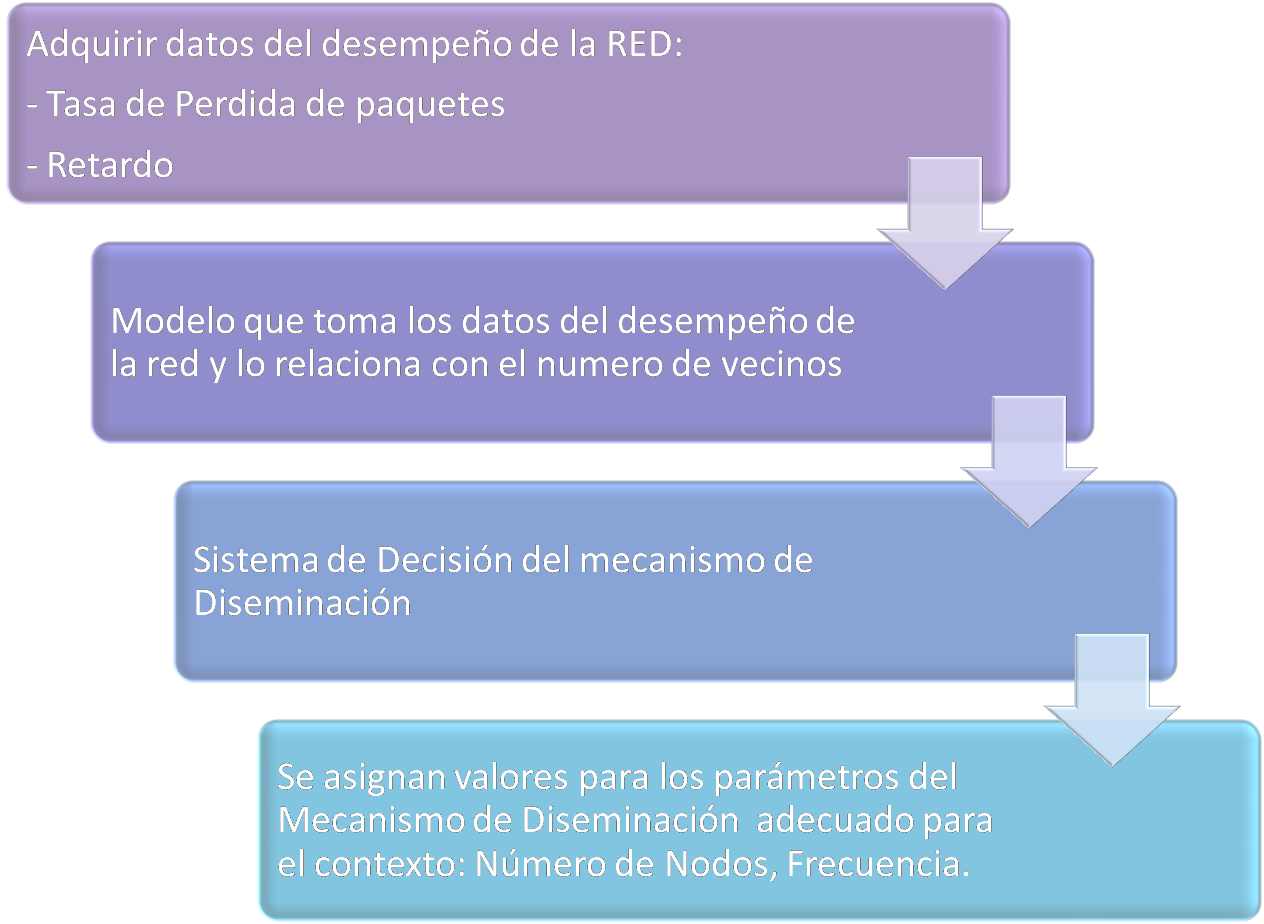
\includegraphics[width=8.5cm]{Diagrama.png}
\caption{Sistema \textit{Context-Aware} Propuesto.}
\label{fig:fig1}
\end{figure}












\chapter{Marco Teórico y Estado del Arte}
\section{Conceptos Técnicos}
En esta sección se presenta y definen los conceptos básicos que permiten el entendimiento de la materia investigada y del posterior trabajo realizado.

\subsection{Redes Vehiculares}

Las redes vehiculares o \textit{Vehicular Networks} en inglés son una nueva clase de redes inalámbricas que han surgido gracias a los avances de las tecnologías inalámbricas y la industria automotriz. Éstas redes son formadas espontáneamente entre vehículos en movimiento equipados con una interfaz inalámbrica (\textit{On Board Units}) que puede ser de tecnología homogénea o heterogéneas. También son conocidas como VANETs (\textit{Vehicular Ad-Hoc Networks}), consideradas la primera aplicación de redes ad-hoc en la vida real, en las cuales se establece comunicación entre vehículos cercanos o con equipamiento fijo en la ruta. %\cite{Moustafa}




\subsection*{Arquitectura de las redes vehiculares}

%\begin{figure}[ht]
%\center
%\includegraphics[width=8.5cm]{ArchVanet.png}
%\caption{Ilustracin de las arquitecturas en redes vehiculares. Fuente}
%\label{fig:fig2}
%\end{figure}


\subsubsection*{Aplicaciones en VANETs}

las cuales se pueden dividir en tres grandes grupos \cite{Bi2017}:

\begin{itemize}
    \item{\textbf{Seguridad en la Ruta}} -- Este tipo de aplicaciones tienen como objetivo reducir los accidentes de tránsito y mejorar la seguridad vial. Por un lado, mediante intercambios de información en tiempo real, los vehículos son capaces de identificar posibles colisiones, e informar a los conductores o iniciar automáticamente los sistemas de control del vehículo para responder a los eventos inminentes. Por otro lado, después de una colisión de vehículos, se produce los intercambios de información en tiempo real, que notifican a otros vehículos para evitar entrar en el lugar peligroso. Por lo tanto, estas aplicaciones de seguridad juegan un papel vital en la reducción de los accidentes de tráfico [24, 25]. Tales aplicaciones tienen requisitos estrictos de retraso de transmisión de mensajes y fiabilidad. En las redes de vehículos, los mensajes de seguridad deben ser entregados a los vehículos cercanos de la manera más rápida y confiable posible.
    
    \item{\textbf{Gestión del tráfico}} -- En la actualidad, la gestión del tráfico en algunas intersecciones importantes en un entorno urbano sigue dependiendo de las intervenciones manuales. Debido a las consideraciones de costos, es difícil lograr una gestión eficiente del tráfico en las carreteras o caminos rurales. Sin embargo, es probable que las direcciones de tráfico soportadas por las comunicaciones vehiculares abarquen más segmentos de carretera, lo que puede mejorar la eficiencia de la gestión del tráfico, reducir la congestión del tráfico y ahorrar tiempo de viaje a los usuarios[26]. Comparado con las aplicaciones de seguridad, este tipo de aplicaciones no tiene requisitos de retraso y fiabilidad, lo que significa que se puede tolerar un pequeño retardo de transmisión o pérdida de paquetes.
    
    \item{\textbf{Entretenimiento}} -- El objetivo de este tipo de aplicaciones es hacer que la vida de los usuarios móviles sea cómoda a través de las comunicaciones vehiculares. Por ejemplo, Los usuarios que viajan pueden disfrutar de servicios multimedia continuos y ubicuos de Internet, por ejemplo, streaming de vídeo, navegación web y descarga de archivos, etc., a través de V2V o V2I en redes vehiculares [27]. Este tipo de aplicaciones tiene requisitos de QoS como la continuidad y alto rendimiento [28].
\end{itemize}

\subsection{DSRC (Dedicated Short-Range Comunication)}

\subsection{Beaconing}

\subsection{Nodos}

2.2.	Redes Móviles
Estas redes son de tipo inalámbrico, es decir el canal físico corresponde al espectro radioeléctrico y requiere de antenas transmisoras y receptoras. Él objetivo de estas redes es que se pueda establecer comunicación con hosts que están constantemente cambiando su posición. 

2.2.1.	Redes Móviles Ad-hoc (MANET)
Estas redes se caracterizan por utilizar una arquitectura P2P, por  lo tanto, la información no viaja hacia un servidor , estableciéndose solo inter-conectividad entre los dispositivos. Las Redes Vehiculares Ad-hoc (VANET) corresponde a un tipo de estas redes  [19].



\section{Revision y Evaluación Crítica del Estado del Arte}

\subsection{Diseminación en VANETs}

\subsection{Mecanismos de Diseminación Escogidos}

\subsection{Detección de Congestión de Tráfico }

Actualmente existen diversas aplicaciones que buscan resolver el problema de la congestión de tráfico a través de sistemas basados en VANETs. Éste se puede dividir en 3 grandes etapas:
\begin{enumerate}
 \item Monitoreo de las principales variables que facilitan la detección de tráfico
 \item Detección o predicción de congestión 
 \item Diseminación eficiente de la información [13].
\end{enumerate}
 
Algunos autores (ver tabla 1) abordan las dos primeras etapas, mientras que otros desarrollan las  3 en plenitud, las cuales pueden  retro-alimentarse, pues, para detectar los nodos vecinos, utilizan una tabla en la cual se indexan la identificación, posición,  velocidad, etc. y en base a esto se puede diseminar la información de manera eficiente, utilizando solo ciertos nodos para retransmitir la información y no sobrecargar el canal de comunicación.
Además las diferentes propuestas se pueden diferenciar en el tipo de variable que utilizan para detectar la congestión de tráfico, algunos utilizan el tiempo de viaje en un segmento de la ruta, mientras que otros utilizan la posición y/o velocidad de vehículos en la vecindad. Estas diferencias se relacionan  con el tipo de arquitectura que utilizan los mecanismos, esta puede ser \textit{V2V}, \textit{V2I-I2V}.
Los sistemas \textit{V2V} se pueden subdividir en aquellos que utilizan un sistema cooperativo distribuido a aquellos que utilizan uno centralizado o aquellos que utilizan un sistema de solicitudes. Las soluciones mas recientes introducen un sistema de diseminación multi-salto, es decir los nodos adquieren la información y la repiten a los nodos vecinos que están mas alejados de la fuente de información. Un resumen compacto del estudio de las propuestas se muestra en la Tabla 1.

\begin{table}[!htb]
\centering
\begin{tabular}{c l c c c}

\hline 
	&	& &Características \\
\hline 
	&Propuestas&	Etapas	&Arquitectura	&Variable utilizada \\
\hline
1&	Lakas (2009). &	1,2,3	& V2V	&Tiempo de Viaje \\
2&	Mohandas (2009). &	1,2,3	&V2I-I2V&	- \\
3&	Bauza (2010). &	1 y 2	&V2V	&Velocidad y Densidad \\
4&	Xu, Y. (2010).& 	1,2,3	&V2V,V2I-I2V	&Velocidad y Densidad \\
5&	Marfia (2011). &	1 y 2	&I2V	&Tiempo de Viaje \\
6&	Singh  (2011). &	1,2,3	&V2V	&Velocidad y Posición \\
7&	Zhang, (2011).& 	1 y 2	&-	&Mapa de Velocidades \\
8	&Terroso-sáenz (2012). 	&1,2,3	&V2V,V2I-I2V&	Velocidad y Posición\\
9&	Xu, Y. (2012).	&1,2,3&	I2V&	Tiempo de Viaje\\
10&Bauza  (2013).& 	1,2,3	&V2V	&Velocidad y Densidad\\
11&	Martuscelli  (2013).&	1,2,3	&V2V&	Posición\\
12	&Younes  (2013). 	&1,2,3	&V2V	&Posición\\
13	&Gramaglia (2014). 	&1,2,3	&V2V&	Posición\\
14	&Milojevic (2014). &	1,2,3&	V2V&	Velocidad y Densidad\\
15&	Shaikh (2014).& 	1,2,3	&V2V&	Velocidad\\
16	&Yuan  (2014). &	1,2,3	&V2V&	Velocidad y Densidad\\
17	&Younes (2015). 	&1,2,3	&V2V&	Velocidad\\
18	&Turcanu  (2016). &	1,2,3	&V2V,V2I-I2V	&Posición\\

\hline

\end{tabular}

\caption{Resumen de las propuestas estudiadas}
\label{tab:tabresumen}
\end{table}


Tanto para detectar como para diseminar  los sistemas basados en beaconing, suelen sufrir desperfectos cuando se tiene congestión de tráfico, debido a la sobrecarga en el canal de comunicación lo que se conoce como tormenta de broadcast. por lo que saber, cuántos vecinos tiene un nodo, en tiempo real y de manera precisa, puede entregar beneficios tanto para la congestión de tráfico como para ajustar los mecanismos de recolección y diseminación de información, además de poder otorgar alternativas a los conductores que prefieren evadir el tráfico, lo puedan hacer manera eficiente. Esto presenta un gran desafío a resolver y explorar en las redes inter-vehiculares, debido a su alto impacto en los tiempos de detección.

\section{Sistemas Context-Aware}


\chapter{Segundo}
\lipsum[50-60]
2.	Marco Teórico

En este capítulo se presenta y definen los conceptos básicos que permiten el entendimiento de la materia investigada y del posterior trabajo realizado.

2.1.	Redes Digitales

A grandes rasgos corresponden  a la conexión  entre dispositivos electrónicos que utilizan un canal para poder intercambiar información relevante para cada uno de estos dispositivos. Esto constituye un sistema de comunicación que utiliza señales digitales y el cual presenta nuevos desafíos, como la discretización y cuantificación de las señales transmitidas, frecuencias de muestreo de señales, formas de hacer uso del canal físico, tecnologías de acceso al medio etc. 

2.2.	Redes Móviles
Estas redes son de tipo inalámbrico, es decir el canal físico corresponde al espectro radioeléctrico y requiere de antenas transmisoras y receptoras. Él objetivo de estas redes es que se pueda establecer comunicación con hosts que están constantemente cambiando su posición. 

2.2.1.	Redes Móviles Ad-hoc (MANET)
Estas redes se caracterizan por utilizar una arquitectura P2P, por  lo tanto, la información no viaja hacia un servidor , estableciéndose solo inter-conectividad entre los dispositivos. Las Redes Vehiculares Ad-hoc (VANET) corresponde a un tipo de estas redes  [19].

2.2.1.1.	Detección de Congestion de Trafico en             VANETs
Actualmente existen diversas aplicaciones que buscan resolver el problema de la congestión de tráfico a través de sistemas de VANETs. Éste se puede dividir en 3 grandes etapas. 1) Monitoreo de las principales variables que facilitan la detección de tráfico, 2) detección o predicción de congestión, y 3) Diseminación eficiente de la información [13]. 
Algunos autores (ver tabla 1) abordan las dos primeras etapas, mientras que otros desarrollan las  3 en plenitud, las cuales pueden  retro-alimentarse, pues, para detectar los nodos vecinos, utilizan una tabla en la cual se indexan la identificación, posición,  velocidad, etc. y en base a esto,  luego se puede diseminar la información de manera eficiente, utilizando solo ciertos nodos para retransmitir la información y no sobrecargar el canal de comunicación.
Además las diferentes propuestas se pueden diferenciar en el tipo de variable que utilizan para detectar la congestión de tráfico, algunos utilizan el tiempo de viaje en un segmento de la ruta, mientras que otros utilizan la posición y/o velocidad de vehículos en la vecindad. Estas diferencias se relacionan  con el tipo de arquitectura que utilizan los mecanismos, esta puede ser V2V, V2I-I2V.
Los sistemas V2V se pueden subdividir en aquellos que utilizan un sistema cooperativo distribuido a aquellos que utilizan uno centralizado o aquellos que utilizan un sistema de solicitudes. Las soluciones mas recientes introducen un sistema de diseminación multi-salto, es decir los nodos adquieren la información y la repiten a los nodos vecinos que están mas alejados de la fuente de información. Un resumen compacto del estudio de las propuestas se muestra en la Tabla 1.

		Caracteristicas
	Propuestas	Etapas	Arquitectura	Variable utilizada
[1]	Lakas (2009). 	1,2,3	V2V	Tiempo de Viaje
[2]	Mohandas (2009). 	1,2,3	V2I-I2V	- 
[3]	Bauza (2010). 	1 y 2	V2V	Velocidad y Densidad
[4]	Xu, Y. (2010). 	1,2,3	V2V,V2I-I2V	Velocidad y Densidad
[5]	Marfia (2011). 	1 y 2	I2V	Tiempo de Viaje
[6]	Singh  (2011). 	1,2,3	V2V	Velocidad y Posición
[7]	Zhang, (2011). 	1 y 2	-	Mapa de Velocidades
[8]	Terroso-sáenz (2012). 	1,2,3	V2V,V2I-I2V	Velocidad y Posición
[9]	Xu, Y. (2012).	1,2,3	I2V	Tiempo de Viaje
[10]	Bauza  (2013). 	1,2,3	V2V	Velocidad y Densidad
[11]	Martuscelli  (2013).	1,2,3	V2V	Posición
[12]	Younes  (2013). 	1,2,3	V2V	Posición
[13]	Gramaglia (2014). 	1,2,3	V2V	Posición
[14]	Milojevic (2014). 	1,2,3	V2V	Velocidad y Densidad
[15]	Shaikh (2014). 	1,2,3	V2V	Velocidad
[16]	Yuan  (2014). 	1,2,3	V2V	Velocidad y Densidad
[17]	Younes (2015). 	1,2,3	V2V	Velocidad
[18]	Turcanu  (2016). 	1,2,3	V2V,V2I-I2V	Posición

Tabla 1. Resumen de las propuestas estudiadas.

Tanto para detectar como para diseminar  los sistemas basados en beaconing, suelen sufrir desperfectos cuando se tiene congestión de tráfico, debido a la sobrecarga en el canal de comunicación lo que se conoce como tormenta de broadcast. por lo que saber, cuántos vecinos tiene un nodo, en tiempo real y de manera precisa, puede entregar beneficios tanto para la congestión de tráfico como para ajustar los mecanismos de recolección y diseminación de información, además de poder otorgar alternativas a los conductores que prefieren evadir el tráfico, lo puedan hacer manera eficiente. Esto presenta un gran desafío a resolver y explorar en las redes inter-vehiculares, debido a su alto impacto en los tiempos de detección.

\begin{conclusion}
	\lipsum[130-132]
	\begin{figure}[!h]
		\centering
		
\includegraphics[scale=.2]{imagenes/fcfm}
		\caption{Logo de la Facultad}
		\label{logofcfm}
	\end{figure}
	\lipsum[133-134]
	\begin{table}[!h]
		\centering
		\begin{tabular}{|c||c|}
			\hline
			Campo 1& Campo 2\\\hline
			Valor 1& Valor2\\\hline
		\end{tabular}
		\caption{Tabla 1}
		\label{tabla:1}
	\end{table}
	\lipsum[135]
\end{conclusion}

% \input{glosario.tex} % opcional

\nocite{*}
\bibliographystyle{plain}
\bibliography{bibliografia}

% \input{anexo_apendices.tex} % opcionales

\end{document}
